\chapter{L'entropie}
Il est intéressant de donner une formulation quantitative au second principe ; 
c'est l'objectif de ce chapitre.

	\section{L'inégalité de Clausius}
	Cette inégalité est un corollaire du second principe :\\
	
	\proposition{Pour tout système fermé à température uniforme décrivant un cycle,
	\begin{equation}
	\oint \dfrac{\delta Q}{T} \leq 0
	\end{equation}
	où $\delta Q$ est la quantité de chaleur reçue sur un élément de cycle, et $T$ 
	la température du système à l'état correspondant.}\ 
	
	\begin{proof}\ \\
	Vérifions cette inégalité sur le cycle de Carnot. Ce cycle réversible : les 
	échanges sont isothermes :
	\begin{equation}
	\oint \dfrac{\delta Q}{T} = \dfrac{Q_C}{T_C} - \dfrac{Q_F^*}{T_F} = 0
	\end{equation}
	L'intégalité est bien vérifiée, toute la source "chaude" va intégralement vers 
	la "froide". Vérifions maintenant que ça soit toujours le 
	cas pour un cycle irréversible\footnote{On considère des parties réversibles, 
	d'autre pas.} : le cycle étant irréversible $W_{irr}^* < W_{rev}^*$ et donc 
	$Q_{F,irr}^* > Q_{F,rev}^*$. On a donc 
	\begin{equation}
	\int_C \dfrac{\delta Q}{T} = \int_C \dfrac{\delta Q}{T_C} = \dfrac{Q_C}{T_C}, 
	\qquad\qquad
	\int_F \dfrac{\delta Q^*}{T} = \int_F \dfrac{\delta Q^*}{T_F} = \dfrac{Q_{F,irr}^*}{T_F} 
	> \dfrac{Q_{F,rev}^*}{T_F} 
	\end{equation}
	On peut directement sortir $Q_C$ de l'intégrale. La dernière inégalité (stricte) 
	provient de l'irréversibilité, provoquant une dégradation de l'énergie. En 
	soustrayant\footnote{L'idée est de faire "apparaître" la relation pour le cycle 
	de Carnot réversible qui est bien nulle en "minorant" l'intégrale.}
	\begin{equation}
	\oint \dfrac{\delta Q}{T} = \int_C \dfrac{\delta Q}{T}-\int_F\dfrac{\delta Q}{T} 
	< \dfrac{Q_C}{T_C}-\dfrac{Q_{F,rev}^*}{T_F} = 0
	\end{equation}
	Un cycle de Carnot frigorifique n'est qu'un cycle de Carnot inversé qui lui 
	aussi satisfait\footnote{On vérifié pour pour un cycle frigorifique, c'est 
	aussi valable pour clore la démonstration.}
	\begin{equation}
	\oint \dfrac{\delta Q}{T} = \dfrac{Q_F}{T_F}-\dfrac{Q_C^*}{T_C} = 0
	\end{equation}
	Ce cycle passe par le même chemin en prélevant la même quantité de chaleur à la 
	source froide $Q_F$ mais avec certaines parties du parcours irréversibles : 
	$W_{irr} > W_{rev} ; Q_{C,irr}^* > Q_{C,rev}^*$. Il en résulte
	\begin{equation}
	\int_F \dfrac{\delta Q}{T} = \int_F \dfrac{\delta Q}{T_F} = \dfrac{Q_F}{T_F}, 
	\qquad\qquad
	\int_C \dfrac{\delta Q^*}{T} = \int_F \dfrac{\delta Q^*}{T_C} = \dfrac{Q_{C,irr}^*}{T_C} 
	> \dfrac{Q_{C,rev}^*}{T_C} 
	\end{equation}
	En 	soustrayant
	\begin{equation}
	\oint \dfrac{\delta Q}{T} = \int_F \dfrac{\delta Q}{T}-\int_C\dfrac{\delta Q}{T} 
	< \dfrac{Q_F}{T_F}-\dfrac{Q_{C,rev}^*}{T_C} = 0
	\end{equation}
	Ce qui complète la démonstration de la proposition.
	\end{proof}
	
	
	\section{L'entropie}
	Soit deux cycles réversibles : $A,B$ ; $A,C$. Comme ils sont réversibles  :
	\begin{equation}
	\oint \dfrac{\delta Q}{T} = \int_1^2 \left(\dfrac{\delta Q}{T}\right)_A + 
	\int_2^1 \left(\dfrac{\delta Q}{T}\right)_B = 0
	\end{equation}
	et
	\begin{equation}
		\oint \dfrac{\delta Q}{T} = \int_1^2 \left(\dfrac{\delta Q}{T}\right)_A + 
	\int_2^1 \left(\dfrac{\delta Q}{T}\right)_C = 0
	\end{equation}
	Après soustraction
	\begin{equation}
	\int_2^1 \left(\dfrac{\delta Q}{T}\right)_B = \int_2^1 \left(\dfrac{\delta 
	Q}{T}\right)_C
	\end{equation}
	Forcément, cette entropie doit être la même : l'intégrale ne dépend pas du 
	chemin parcouru et ça sent bon pour formé une variable d'état (différentielle 
	exacte).\\
	La relation suivante est importante, car elle indique que la différence entre 
	deux états n'est pas fonction du parcours (réversible ou non) \textbf{mais} 
	pour calculer cette différence il faut imaginer un parcours réversible et 
	calculer :
	\begin{equation}
	dS = \left(\dfrac{\delta Q}{T}\right)_{rev}
	\end{equation}
	il s'agit de l'\textbf{entropie}. Si le parcours n'est pas réversible, on ne 
	sait pas comment $T$ varie et on ne peut pas calculer !
	
	\section{L’entropie d’une substance pure}
	On peut rentre l'entropie, extensive, en une variable intensive : l'entropie 
	massique $s$. On la lie au titre par la relation
	\begin{equation}
	s = (1-x)s_l + xs_g = s_l + x(s_g-s_l)
	\end{equation}
	
	
	\section{Les variations d’entropie au cours de transformations réversibles}
		\subsection{Le cycle de Carnot}
		Le cycle de Carnot se décompose en quatre transformations
		\begin{enumerate}
		\item \textit{Chauffage isotherme}.\\
		On a 
		\begin{equation}
		S_2-S_1 = \int_1^2 \dfrac{\delta Q}{T} = \dfrac{_1Q_2}{T_C}
		\end{equation}
		avec $_1Q_2$ l'aire $1-2-b-a-1$.
		\item \textit{Détente adiabatique}.\\
		Adiabatique et réversible, $dS=0$. Le segment vertical $2-3$ est dit 
		isentropique.
		\item \textit{Refroidissement isotherme}.\\
		Comme pour 1-2, on a
		\begin{equation}
		S_4-S_3 = \int_3^4 \dfrac{\delta Q}{T} = \dfrac{_3Q_4}{T_4}
		\end{equation}		
		grandeur négative car $_3Q_4<0$. La chaleur cédée à la source froide est 
		l'aire $3-4-a-b-3$.
		\item \textit{Compression adiabatique}.\\
		Même topo, $dS=0$.
		\end{enumerate}
		Le travail net du cycle $W^*$ valant la chaleur nette reçue, il correspond 
		à l'aire $1-2-3-4$ et exprimer le rendement 
		\begin{equation}
		\epsilon_{th} = \dfrac{W^*}{Q_C} = \frac{\text{aire} 1-2-3-4-1}{\text{aire} 
		1-2-b-a-1}
		\end{equation}
			\begin{center}
	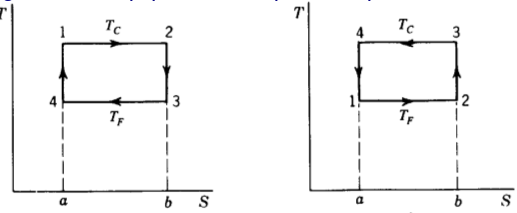
\includegraphics[scale=0.45]{ch7/image1.png}
	\captionof{figure}{Cycles de Carnot (normal et frigo)}
	\end{center}
		Inverser le sens de parcours donne le cycle de Carnot frigorifique.
		
		\subsection{Le chauffage isobare}
		\begin{wrapfigure}[10]{l}{4cm}
		\vspace{-5mm}
		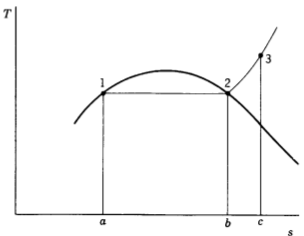
\includegraphics[scale=0.35]{ch7/image2.png}
		\captionof{figure}{ }
		\end{wrapfigure}
		Chauffons de façon isobare réversible une masse de fluide  :
		\begin{equation}
		s_2-s_1 = s_g-s_l = \dfrac{1}{m}\int_1^2 \dfrac{\delta Q}{T} = \dfrac{1}{m}
		\int_1^2 \delta Q = \dfrac{_1q_2}{T} = \dfrac{h_g-h_l}{T}
		\end{equation}
		car pour une isobare en système fermé $\Delta q = \Delta h$. Cette chaleur 
		correspond à l'aire $1-2-b-a-1$. Si on chauffe jusqu'à l'état de vapeur ($2-3$) :
		\begin{equation}
		_2q_3 = \int_2^3 Tds
		\end{equation}
		ce qui est assez délicat à intégrer.
	
	
	
	
	
	
	
	
	
	
	
	
	
	
	
	
	
	
	
	
	
	
	